%!TEX root = ../template.tex
%%%%%%%%%%%%%%%%%%%%%%%%%%%%%%%%%%%%%%%%%%%%%%%%%%%%%%%%%%%%%%%%%%%%
%% chapter4.tex
%% NOVA thesis document file
%%
%% Chapter with lots of dummy text
%%%%%%%%%%%%%%%%%%%%%%%%%%%%%%%%%%%%%%%%%%%%%%%%%%%%%%%%%%%%%%%%%%%%

\typeout{NT FILE chapter4.tex}%

\chapter{Evaluation}
\label{cha:evaluation}

\section{Benchmark platform} % (fold)
\label{sec:benchmark_platform}

It was constructed a benchmark platform to compare our solution to existing ones.
This section discusses the proposed benchmark platform's requirements and design.
\citeauthor{microservices2017benchmark} \cite{microservices2017benchmark} propose an initial set of requirements
to support repeatable microservices research (Figure \ref{fig:benchmark}).

\begin{figure}[htbp]
    \centering
    \centerline{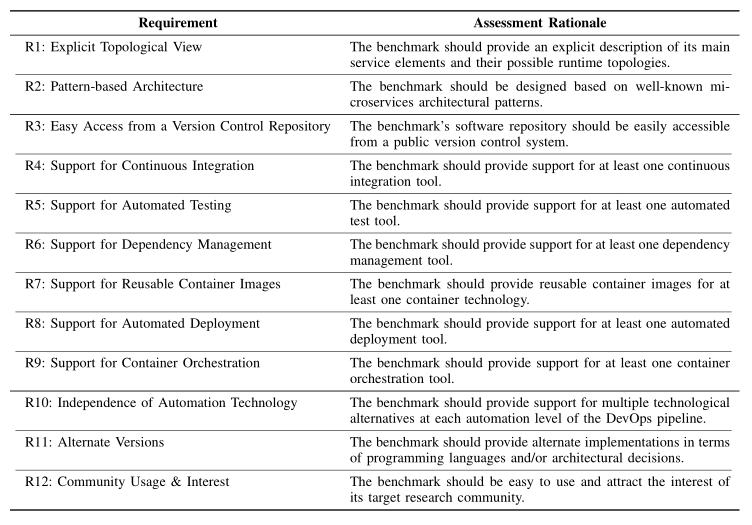
\includegraphics[height=4.2in]{benchmark_requirements}}
    \caption{Benchmark requirements \cite{microservices2017benchmark}}
    \label{fig:benchmark}
\end{figure}

In addition to the requirements listed above, it was considered that the following requirements should also be included:
\begin{itemize}
    \setlength\itemsep{0em}
    \item The ability to evaluate different solutions in comparable scenarios while utilizing the same evaluation criteria;
    \item The ability to evaluate diverse solutions without changing their implementation;
    \item Experiments must be easy to share and replicate;
    \item It should be possible to aggregate reported metrics for a specific time period between two events, such as the start and end of a service's evolution;
    \item Users must be able to specify how and when each service should evolve via a configuration file or directly through a terminal.
\end{itemize}

The architecture of the benchmark platform can be seen in Figure \ref{fig:benchmarkarchitecture}, and its components are described subsequently.

\begin{figure}[htbp]
    \centering
    \centerline{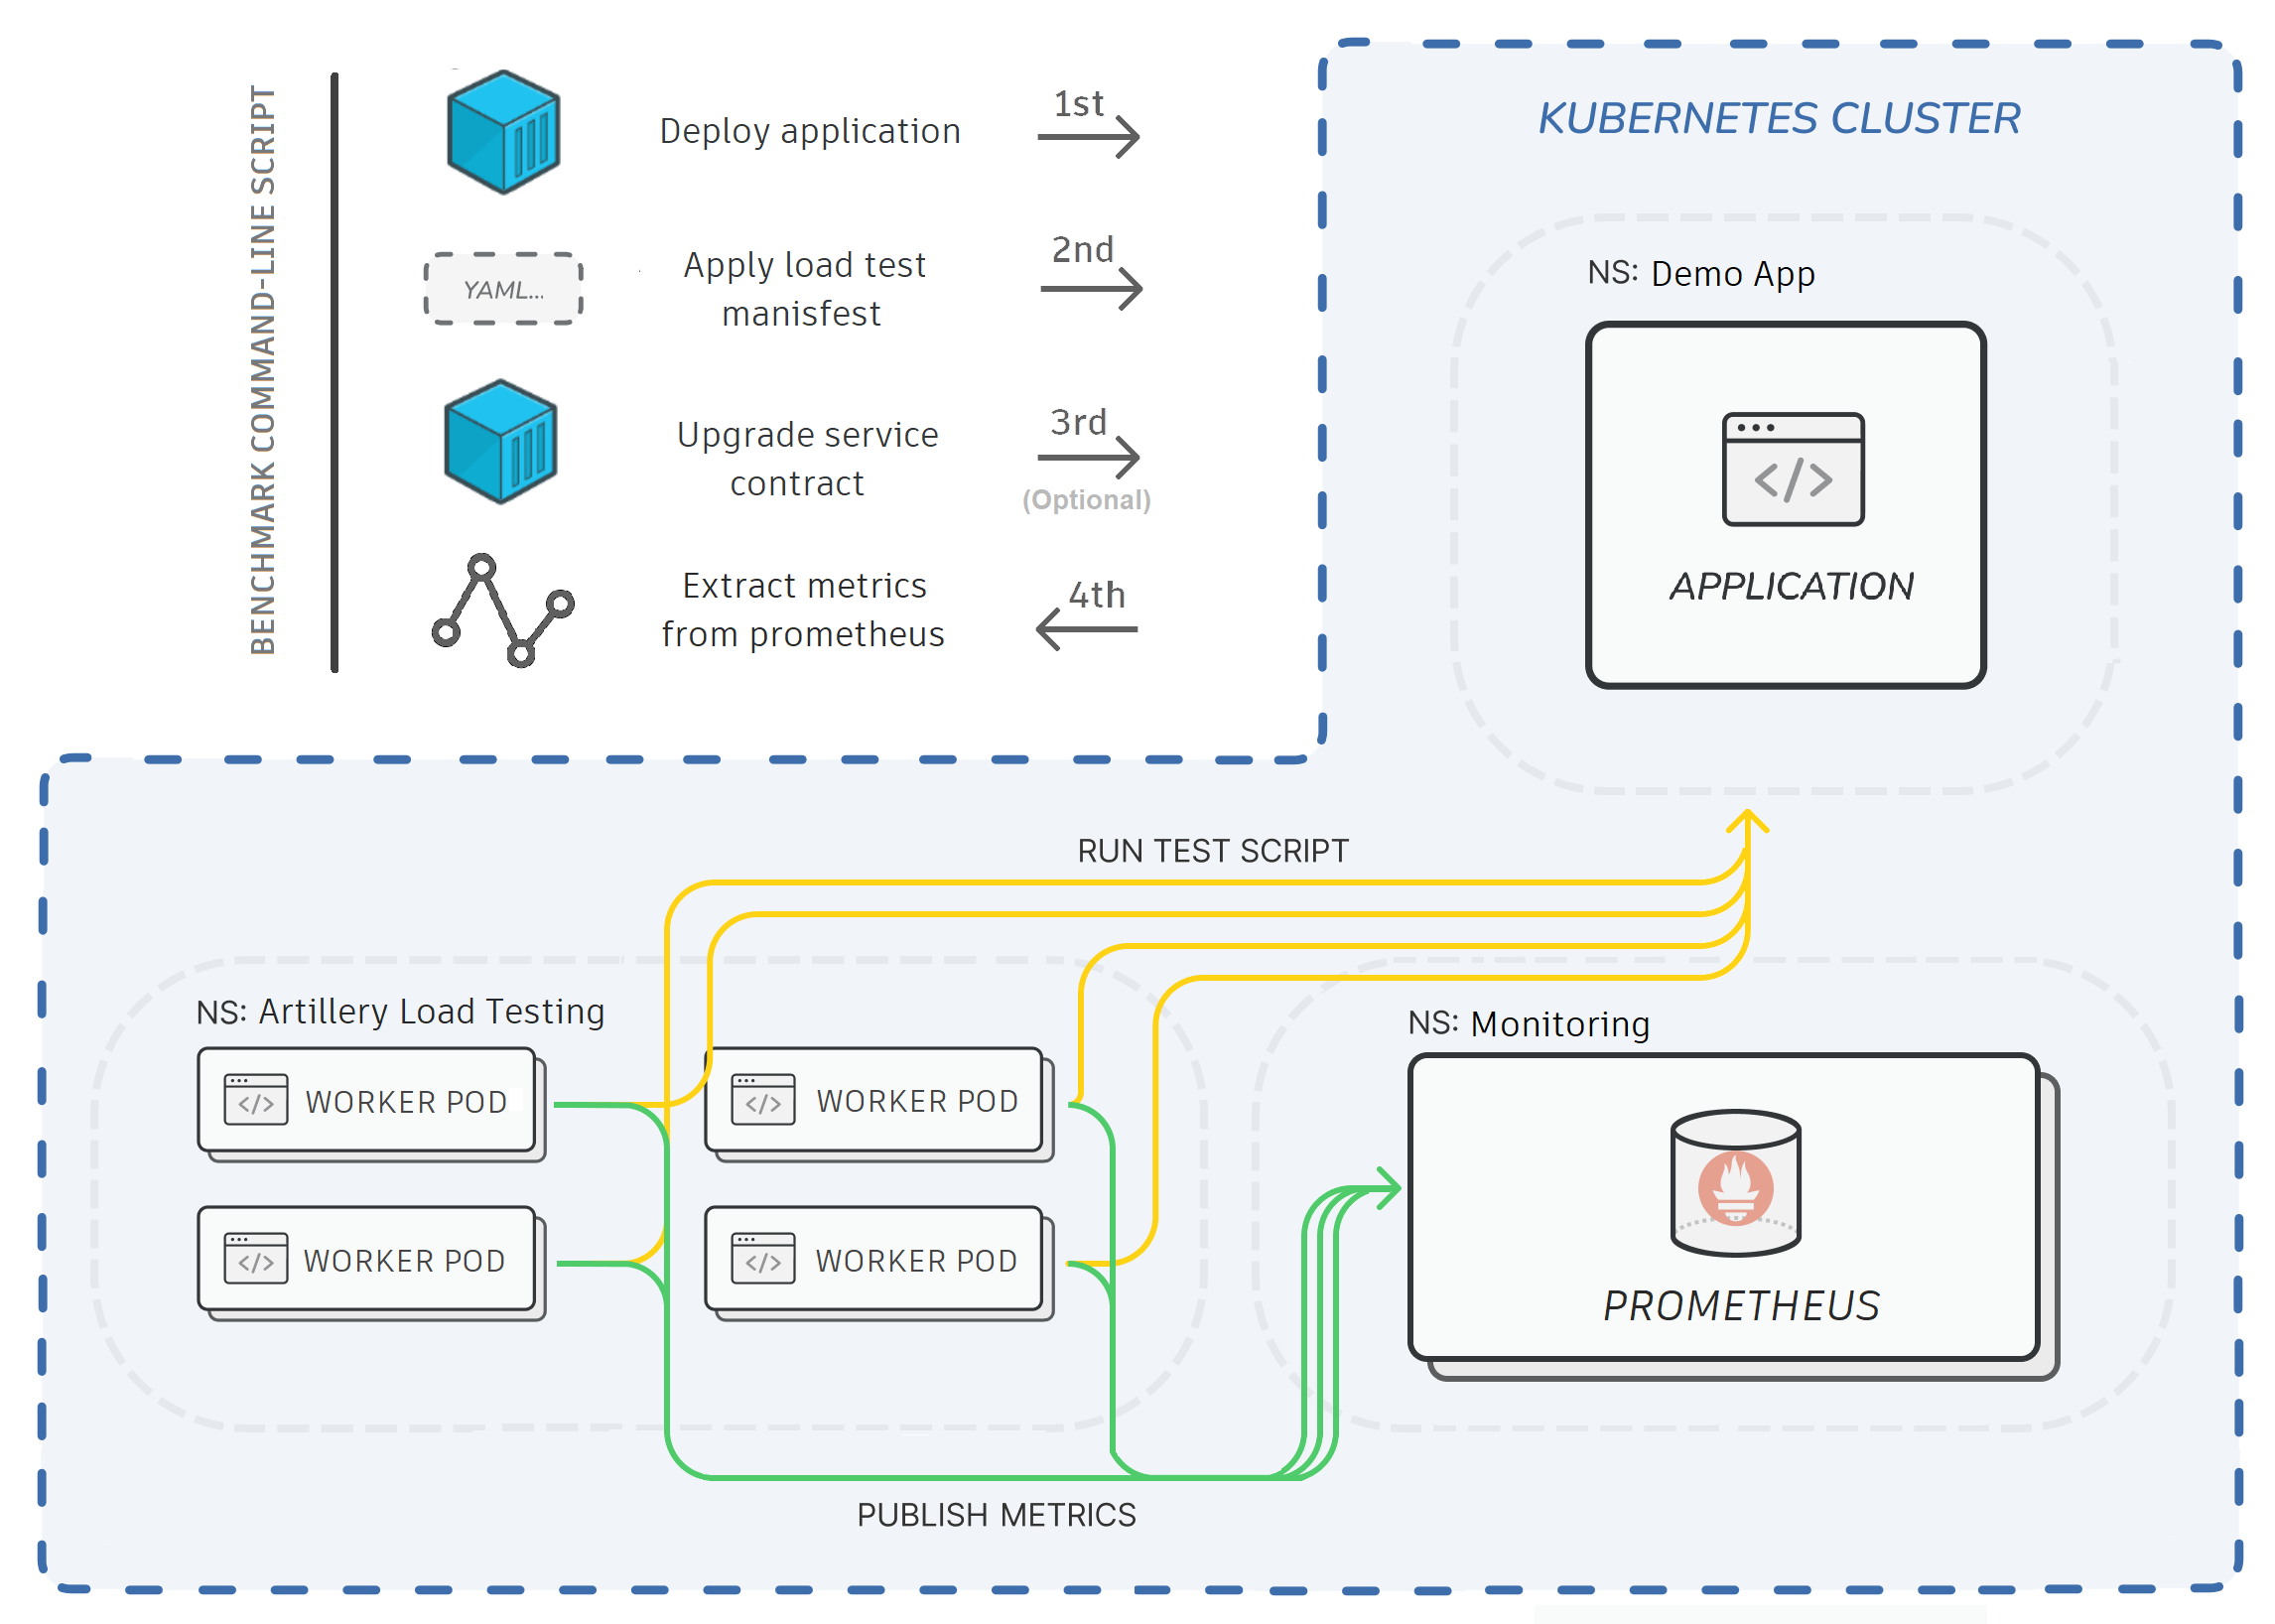
\includegraphics[height=4.2in]{benchmark-architecture}}
    \caption{Benchmark platform architecture}
    \label{fig:benchmarkarchitecture}
\end{figure}

\paragraph{- Kubernetes \cite{kubernetes} -} is the test environment.
It hosts the applications under test, the monitoring system, and the load test workers.

\paragraph{- Promotheus \cite{turnbull2018monitoring} -} is a pull-based monitoring system.
It periodically sends HTTP scrape requests, the response to these requests is parsed in storage along with the metrics for the scrape itself.
Prometheus provides a query language that allows the metrics to be aggregated by events, components or metadata.
The gathered metrics can be consulted by external tools or directly visualized in this platform via dashboards.

\paragraph{- Artillery \cite{artillery} -}
is an open-source load testing suite for developers and system administrators.

\paragraph{- Artillery Operator \cite{artilleryop} -}
enables the creation and execution of distributed Artillery load tests from Kubernetes schedule jobs.
The architecture of this tool is depicted in Figure \ref{fig:artilleryoperator}.

\paragraph{- Helm \cite{helm} -}
is a package manager for Kubernetes that allows developers to more easily deploy, package, and configure applications into Kubernetes clusters.

\paragraph{- Helmfile \cite{helmfile} -}
 extends Helm's capabilities by enclosing it in a declarative specification that allows the composition of multiple Helm charts as a single deployment artifact.

\begin{figure}[htbp]
    \centering
    \centerline{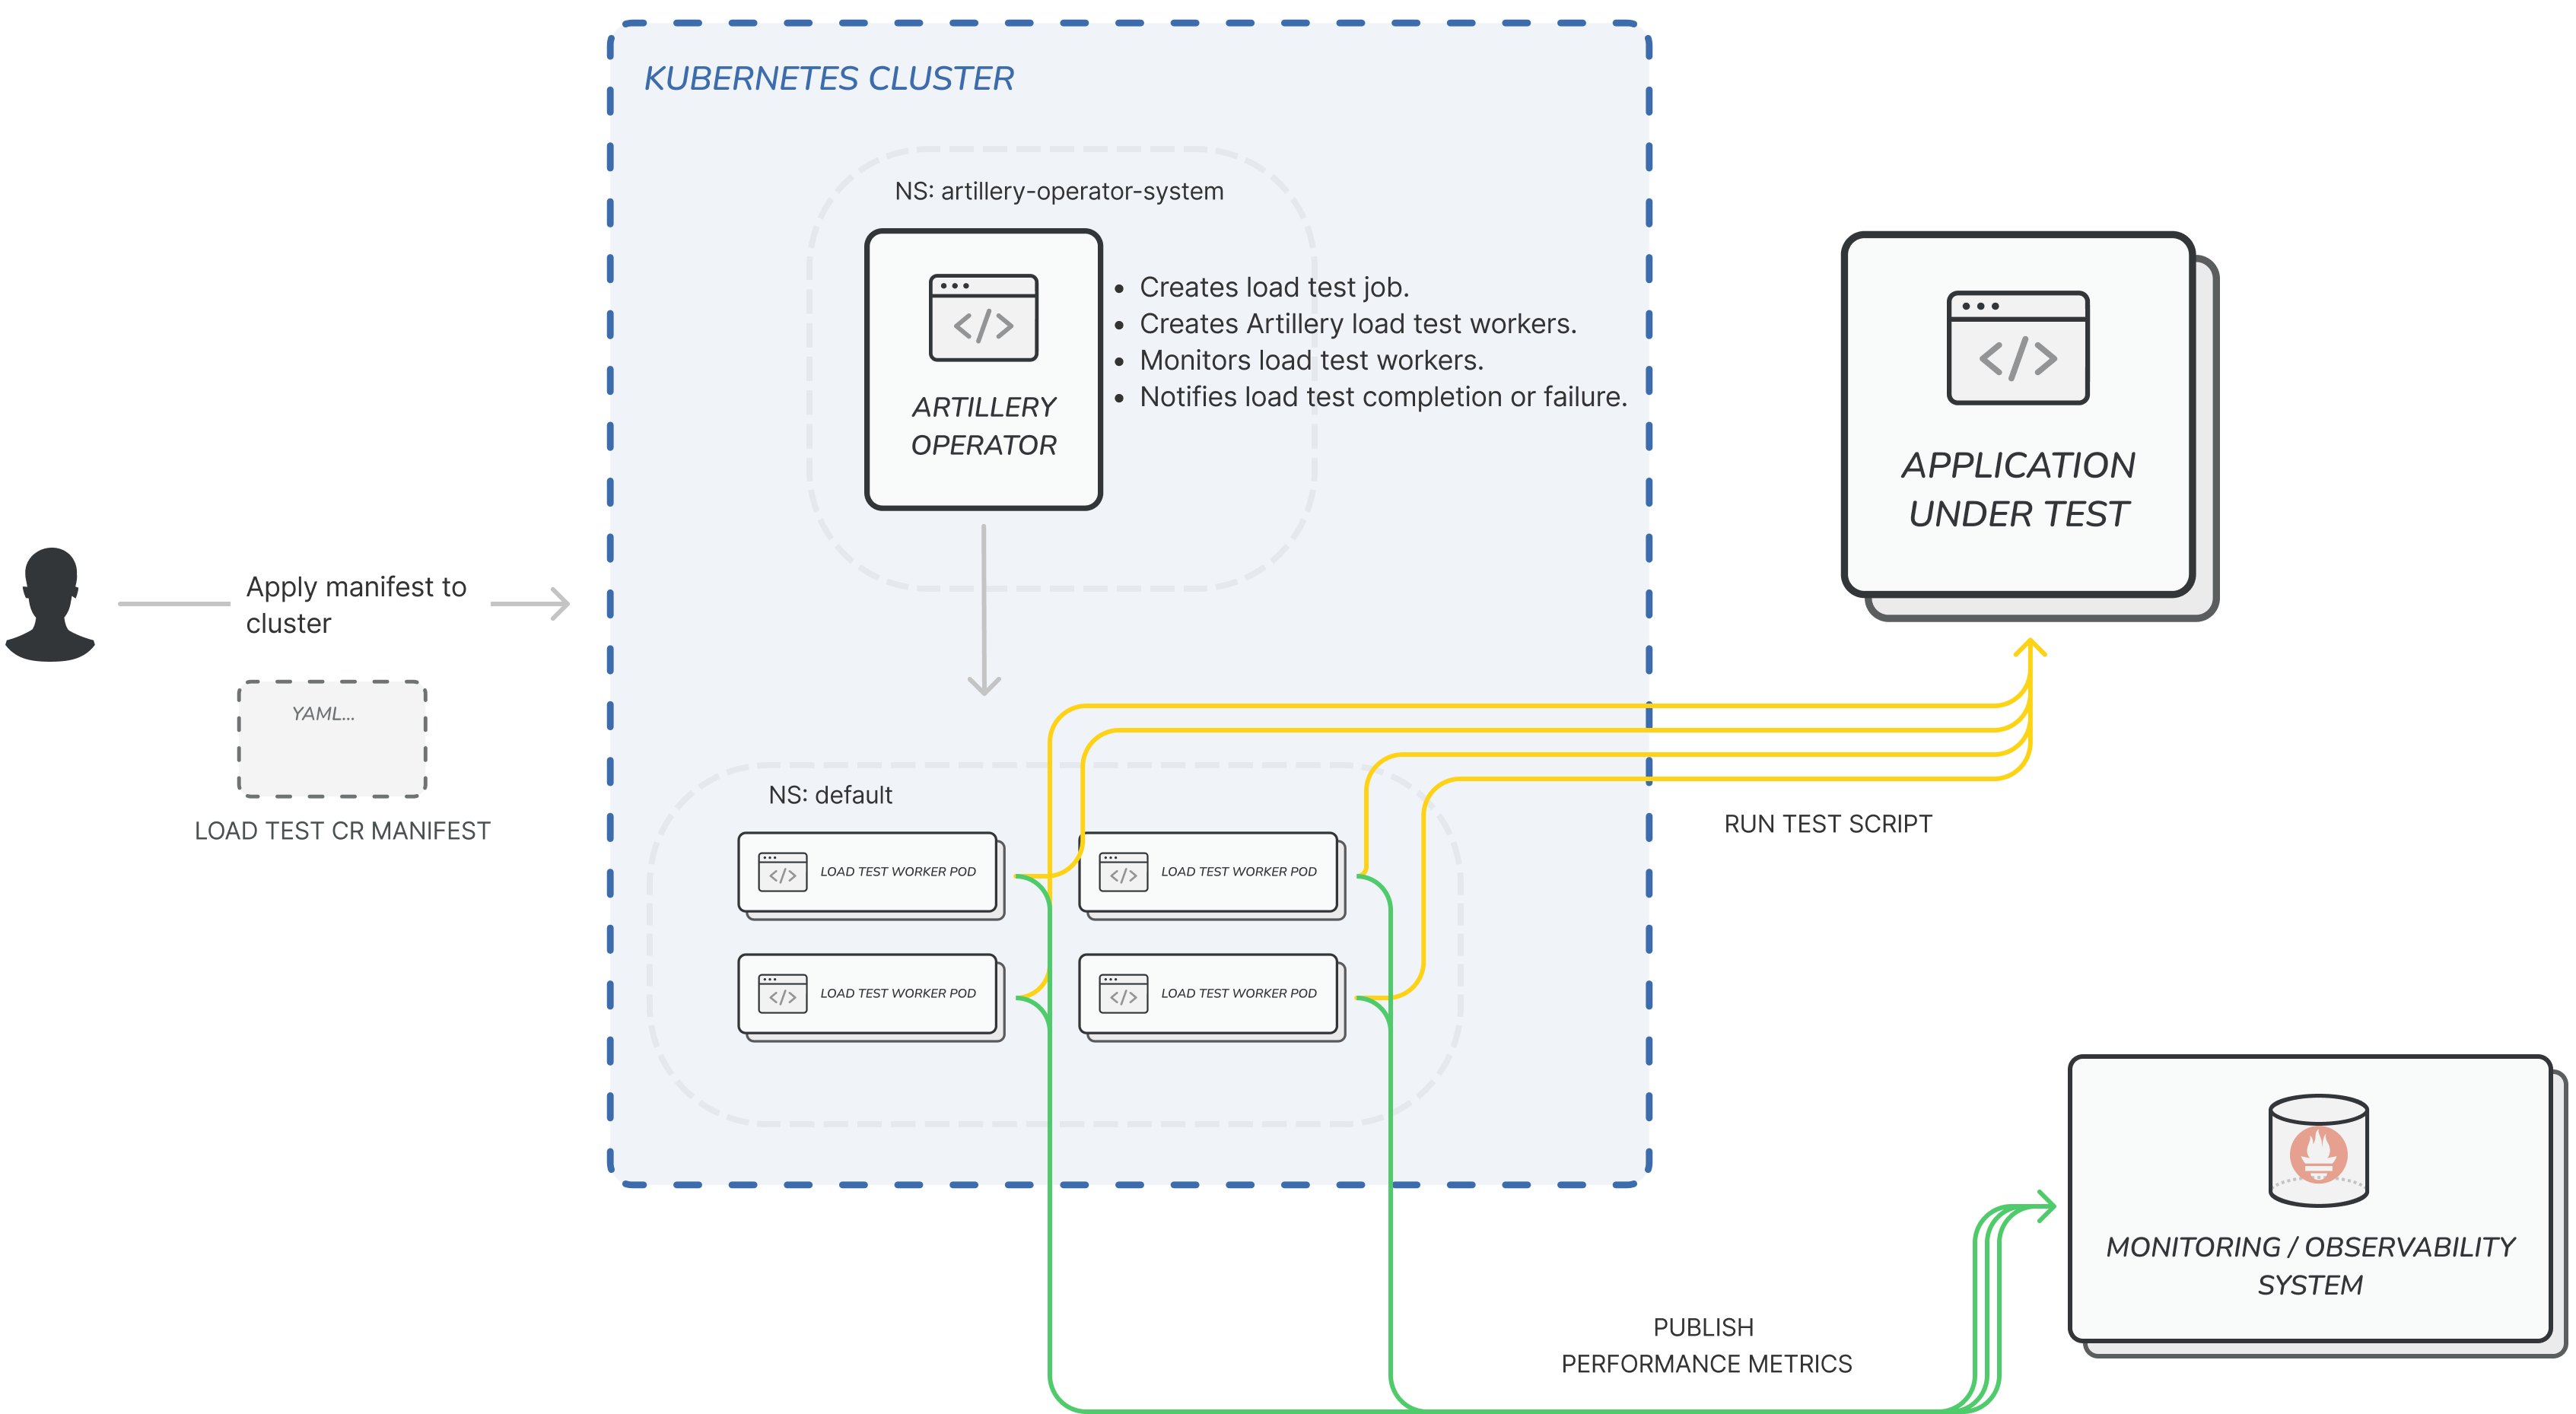
\includegraphics[height=4.2in]{artillery-operator-architecture}}
    \caption{Artillery operator architecture}
    \label{fig:artilleryoperator}
\end{figure}

Experiments are launched using a custom command-line tool.
The command-line tool can also be used to install all the benchmark platform's required components in a Kubernetes cluster.
The tool allows for the execution of multiple experiments in sequence without the need for developer intervention.
The components and resources of an experiment are automatically deleted, and experiment metrics are automatically gathered at the end of the experiment.
The experiment metrics are obtained by querying the prometheus monitoring system, which returns a series of the observations recorded throughout the experiment.
An experiment is composed by four manifests:
\begin{itemize}
    \setlength\itemsep{0em}
    \item \textbf{Helmfile} specifies the resources, and the configuration of the application under test;
    \item \textbf{Artillery workload job} defines the test scenarios of the experiment;
    \item \textbf{Metrics script} holds the queries that should be performed after the experiment ends;
    \item \textbf{(Optional) Evolution script} outlines the deployment actions required to upgrade services during the experiment execution.
\end{itemize}

Each of the four manifests can include template variables that are changed using a configuration file.
An experiment is started by passing the configuration file to a run script.
The developed demo application and load test scripts support the following configurations:
\begin{itemize}
    \setlength\itemsep{0em}
    \item Warm up phase duration;
    \item Ramp up phase duration;
    \item Sustained load phase duration;
    \item Warm up arrival rate;
    \item Ramp up phase min arrival rate;
    \item Ramp up phase max arrival rate;
    \item Sustained load phase arrival rate;
    \item Number of distributed artillery workers;
    \item Number of application replicas;
    \item Payload size of the sent messages;
    \item Recursion - Number of subsequent blocking calls after an initial request;
    \item Fanout - Number of parallel calls for a single request.
\end{itemize}

\section{Evaluation Methodology} % (fold)
\label{sec:evaluation_methodology}

The setup and the methodology of the conducted experiments is described below:

\paragraph{- Environment -}

The experiments were conducted in a cloud environment with 10 virtual machines.
All 10 nodes were hosted in the same datacenter in the region of Strasbourg, France.
Each virtual machines was hosted in different physical machines, no two VMs shared the same hardware.
Each node is interconnected with a bandwidth of 2 Gb/s.
Each virtual machine is equipped with 4GB of RAM and 2 virtual cores of an Intel Core Haswell (no TSX) CPU.

\paragraph{- Tested microservice system -}

To test the cost of the adapter system a demo application was developed.
The demo application holds a configurable amount of services that run an identical image.
The image is a simple HTTP spring server that returns received requests unchanged.
The interconnections between microservices is configurable thorough environment variables.
The number of synchronous calls (SyC) between microservices for a single request and also the number of parallel calls (PrC) between microservices is configurable.
The demo application was developed in two separate versions with unique contracts.
In the first version, one of the procedures of the application was altered.
All the parameters in the body's schema of this procedure were renamed.

\paragraph{- Experiment Setup -}

To inject load in the experiments, 10 workers of the artillery load testing tool were used,
the workers are executed remotely in the cluster and were spread in 6 nodes.
These workers are supported by Kubernetes pods that are monitored by a common job.
The workers are installed and removed from cluster using the artillery-operator project \cite{artilleryoperator}.
In each experiment all the resources of previous experiments were deleted and a new job and namespace were created in the
cluster to avoid contamination in the metrics extracted.
The experiments were carried out sequentially with a 5 minutes break in between.

Each experiment had three phases:
a warm up phase of 30 seconds with an arrival rate of 5 virtual users/second;
a ramp up phase of 2 minutes;
a sustained load phase of 6 minutes.
The metrics were only extracted during the sustained load phase.
The first and last 30 seconds were left out to allow time for all the artillery worker threads to enter the sustained load phase.
It was excluded tests that had a high enough throughput to saturate the application.
The error rate and timeouts were 0 during all the presented experiments.

\paragraph{- Metrics -}

In each experiment it was extracted 3 metrics: the CPU resources, the memory resources and latency of the system.
The resources were only queried from the adapters and the replicas that belong to the target microservice application under test.
The resources consumed by the monitoring system and artillery workers were excluded from the results.
The throughput and latency were extracted by parsing the reports of the artillery load testing tool.
The CPU resource samples were taken from each node at 5 seconds intervals using the prometheus node exporter.
Memory resource samples were gathered from each container at 5 seconds intervals using the kubelet node agent API.
The latency statistics were calculated with a period of 10 seconds over 5 minutes, the results obtained represent the
average of the reported 30 periods.

\section{Experiments} % (fold)
\label{sec:experiments}

Four experiments were carried out in order to test the implementation of the prototype:
the point-to-point experiment, the weighted point-to-point experiment, the bi-partition experiment, and the live contract evolution experiment.
The experiments are detailed below.

\subsection{Point to Point Experiment}

The topology of this experiment is represent in Figure \ref{fig:point}.
The primary goal of this experiment was to assess the overhead of the adapter in terms of latency and computational resources.

\begin{figure}[htbp]
    \centering
    \centerline{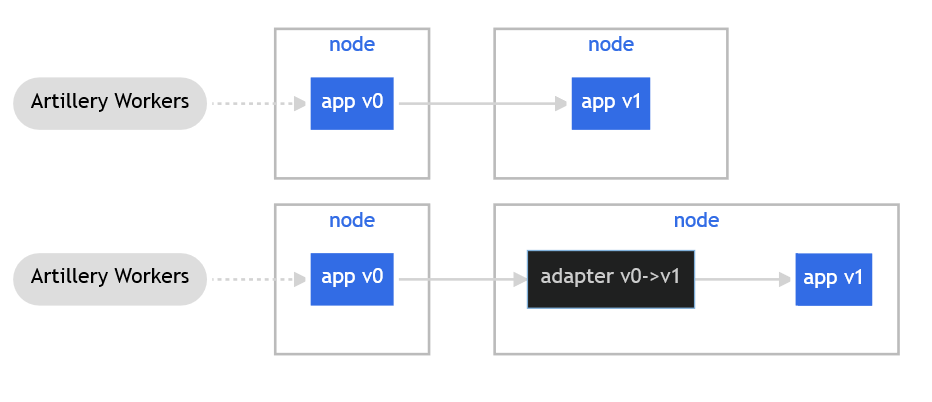
\includegraphics[height=2.4in]{pointExperiment}}
    \caption{Point-to-point experiment}
    \label{fig:point}
\end{figure}

The experiment is composed by two microservices:
the first receives requests from artillery workers and forwards them to the second microservice, which responds with the request.
It was first established a baseline of comparison
by doing the tests without the adapter, and then, the adapter was introduced and the tests were repeated.

The measured CPU overhead of the adapter over a
range of request rates is depicted in Figure \ref{fig:cpuPtp}.
The overhead was calculated by processing the averages of the measured CPU resources in the baseline and adapter tests, and then by dividing the two averages.

\begin{figure}[htbp]
    \centering
    \centerline{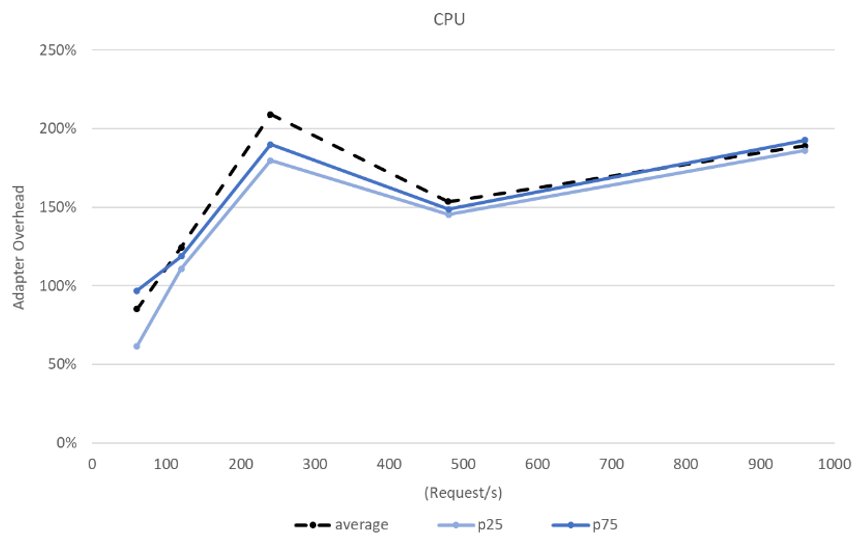
\includegraphics[height=3.5in]{Results/PtP/Cpu-PtP}}
    \caption{Adapter CPU overhead in the point-to-point experiment - 100 bytes (payload size)}
    \label{fig:cpuPtp}
\end{figure}

In this experiment it is expected to have an overhead of 150\% because: the adapter and the microservices share the same request rate;
the cost of the adapter is expected to be equal or to the cost of the tested microservices.
The tested microservices were implemented with the same frameworks as the adapter, consequently adding the adapter will be equivalent to adding one more microservice to the existing two.

The overhead 84\% in first data point is explainable by the configuration of the containers:
the adapter and demo application containers were initialized in Kubernetes with a default of 100 millicpu (1000 millicpu is equivalent to 100\% of a CPU core),
this CPU resources far exceed the capacity necessary to support a request rate 60 requests/second,
consequently the container's CPU scheduling was throttle-down after start up;
the overhead was inferior to 100\% because the scheduled CPU resources in the experiment with the adapter, were throttled down faster than in the baseline experiment without the adapter.
As can be seen in the results shown Figure \ref{fig:cpuPtp} the measured overhead doesn't fall to far outside our expectations.

Figure \ref{fig:memPtp} shows the measured memory overhead of the adapter over a
range of request rates.
The overhead was calculated by processing the averages of the measured memory resources in the baseline and adapter tests, and then by dividing the two averages.

The average cost of 190\% in Figure \ref{fig:memPtp} is understandable because: although being stateless, the adapter stores two transient messages in memory for each request, the request message and the adapted request message;
the demo application only keeps one request in memory, it stands to reason that the adapter memory cost is roughly double of the demo application.
As can be seen in Figure \ref{fig:memCostPtp}, the used memory of the adapter grows linearly with the request rate, as it was expected.

\begin{figure}[htbp]
    \centering
    \centerline{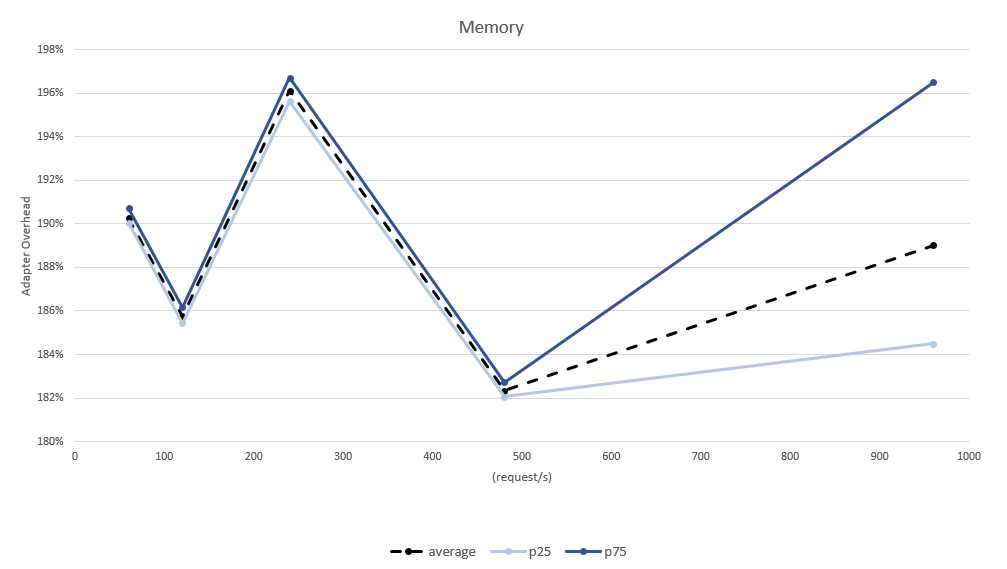
\includegraphics[height=3.3in]{Results/PtP/Memory-PtP}}
    \caption{Adapter memory overhead in the point-to-point experiment - 100 bytes (payload size)}
    \label{fig:memPtp}
\end{figure}

\begin{figure}[htbp]
    \centering
    \centerline{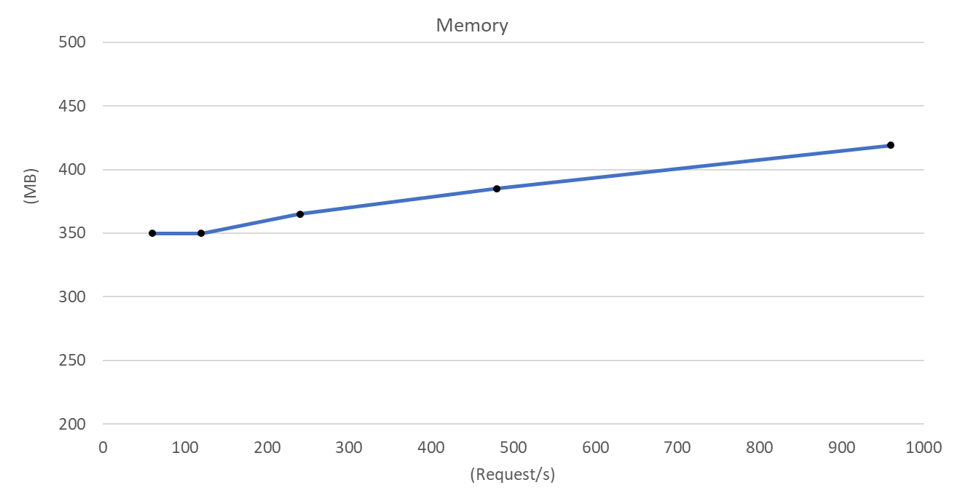
\includegraphics[height=3in]{Results/PtP/MemoryCost_PtP}}
    \caption{Adapter memory cost in the point-to-point experiment - 100 bytes (payload size)}
    \label{fig:memCostPtp}
\end{figure}

\newpage

The latency overhead of the adapter in the point-to-point experiment is depicted in Figure \ref{fig:latPtP}.
The overhead was calculated by processing the averages of the measured latency in the baseline and adapter tests, and then by dividing the two averages.

\begin{figure}[htbp]
    \centering
    \centerline{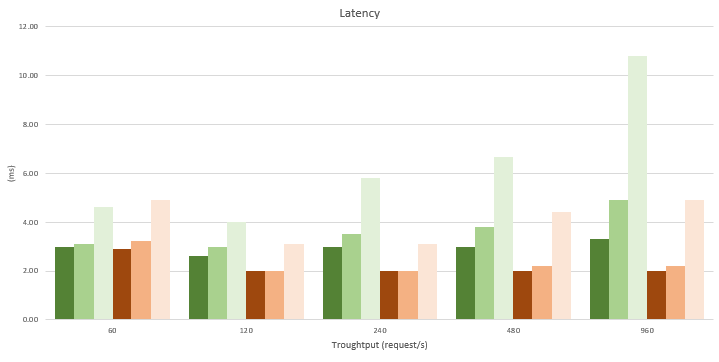
\includegraphics[height=3.5in]{Results/PtP/Latency-PtP}}
    \caption{Adapter latency cost in the point-to-point experiment - 100 bytes (payload size)}
    \label{fig:latPtP}
\end{figure}

It is expected for the overhead to be less or equal to 150\%, because the latency overhead is largely attributable to communication costs.
The adapter introduces an additional communication step ''app1\textrightarrow adapter\textrightarrow app2'' to the baseline communication chain that already has two steps ''workers\textrightarrow app1'' and ''app1\textrightarrow app2''.
The introduced communication step is expected to have a slightly inferior cost to the other steps, as it is performed via interprocess-calls, while the others are done via a private network with 2 GB of bandwidth.
The hypothesis is confirmed by the experiment results in Figure \ref{fig:latPtP}.

The Figures  \ref{fig:payloadCpuPtP} and \ref{fig:payloadLatPtP} illustrate how larger payload sizes effect the latency and the consumed CPU resources.
A request rate of 480 request per second was used in this experiment.
The latency is expected to rise with larger payload sizes because the HTTP packet size is typically 1.5 KB, bigger messages will need to be sent in multiple packets.
The CPU cost is also expected to rise because the cost of deserialization of messages grows with the message payload size.

\begin{figure}[htbp]
    \centering
    \centerline{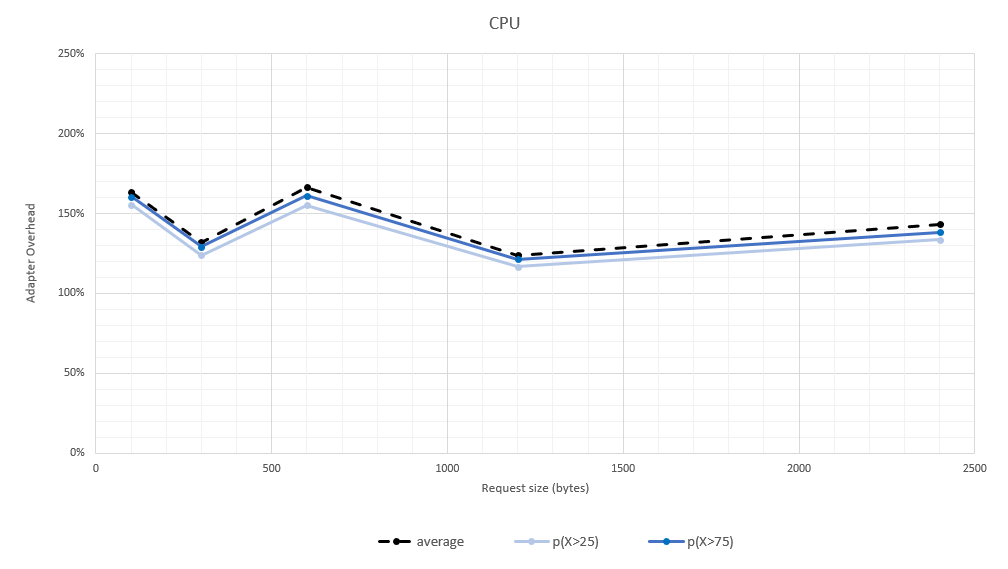
\includegraphics[height=3.5in]{Results/PtP_Size/Cpu-PtP_Size}}
    \caption{Adapter CPU cost in the point-to-point experiment - 480 request/s (arrival rate)}
    \label{fig:payloadCpuPtP}
\end{figure}

\begin{figure}[htbp]
    \centering
    \centerline{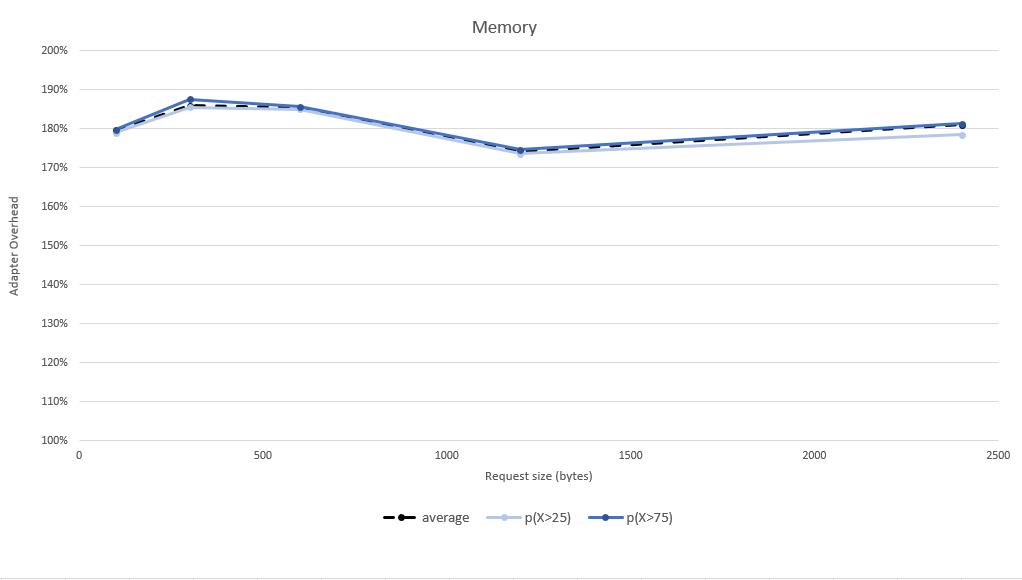
\includegraphics[height=3.5in]{Results/PtP_Size/Latency-PtP_Size}}
    \caption{Adapter Latency cost in the point-to-point experiment - 480 request/s (arrival rate)}
    \label{fig:payloadLatPtP}
\end{figure}

The results illustrated don't reveal any difference for the tested range of payload sizes.
This can be explainable because the tested payload size range of 100 bytes to 2 KB each fits under a single HTTP packet.
This range has initially selected because most services use HTTP messages that fall under this range.
In future work this experiment should be repeated for larger payload sizes, up to 2 MB, to see how the adapter scales in this scenario.

\subsection{Weighted Point to Point Experiment}

The topology of this experiment is represent in Figure \ref{fig:routExp}.
This experiment is also composed by the two microservices, where the first microservice forwards a percentage of its request thorough the adapter
and forwards its remaining requests directly to the other microservice.
The primary goal of this experiment was to see if the adapter overhead is significantly lower in scenarios where only a small percentage of all requests require adaptation.

\begin{figure}[htbp]
    \centering
    \centerline{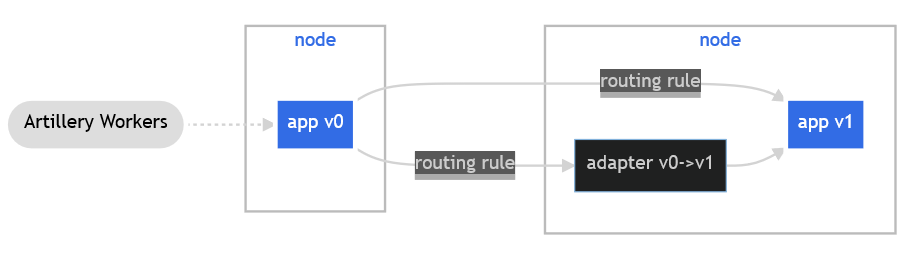
\includegraphics[height=1.7in]{routingExperiment}}
    \caption{Weighted point to point experiment}
    \label{fig:routExp}
\end{figure}

Figure \ref{fig:routCpu} depicts the measured CPU cost of the adapter, the horizontal axis represents the percentage of requests that need adaptation, and the vertical axis represents the
CPU cores utilized by the adapter and demo applications.

\begin{figure}[htbp]
    \centering
    \centerline{\includegraphics[height=2.9in]{Results/R/Cpu-R}}
    \caption{CPU used in the routing experiment - 480 request/s (arrival rate) 100 bytes (payload size)}
    \label{fig:routCpu}
\end{figure}

In this experiment it is expected for the overhead to steadily increase because the arrival rate will increase, as the adapter receives a higher percentage of requests. To support higher request rates
the adapter implementation will need to launch more client threads which, consequently, increase the consumed CPU resources.

When comparing the first and last data points in Figure \ref{fig:routCpu}, we can see that consumed resources have doubled, as expected.
In the other data points, the overhead remains relatively constant with a margin of error of 20\%,
this explainable because the default amount of allocated threads by Tomcat (200 threads) is sufficient to handle the arrival rate in these data points.
When 50\% of requests are routed through the adapter, the arrival rate is 240 requests/s, the tomcat thread model uses a thread per request,
consequently 240 threads are necessary to handle the arrival rate, which can be translated to an overhead of 120\%.

The 20\% margin of error in the other data points is explainable by the nondeterministic nature of the artillery workers.
Remark that the artillery test has two scenarios: one where the worker calls an endpoint that can only be handled by using the adapter, and another in which the adapter is not utilized.
Each scenario weight as set to reflect the corresponding test percentages,
however, the distribution of requests is nondeterministic and will only be equal to the given weights over very long test periods.
The test time for this experiment was set to 5 minutes for each data point.

The utilized memory of the adapter and demo applications in this experiment is depicted in Figure \ref{fig:routMem}.

\begin{figure}[htbp]
    \centering
    \centerline{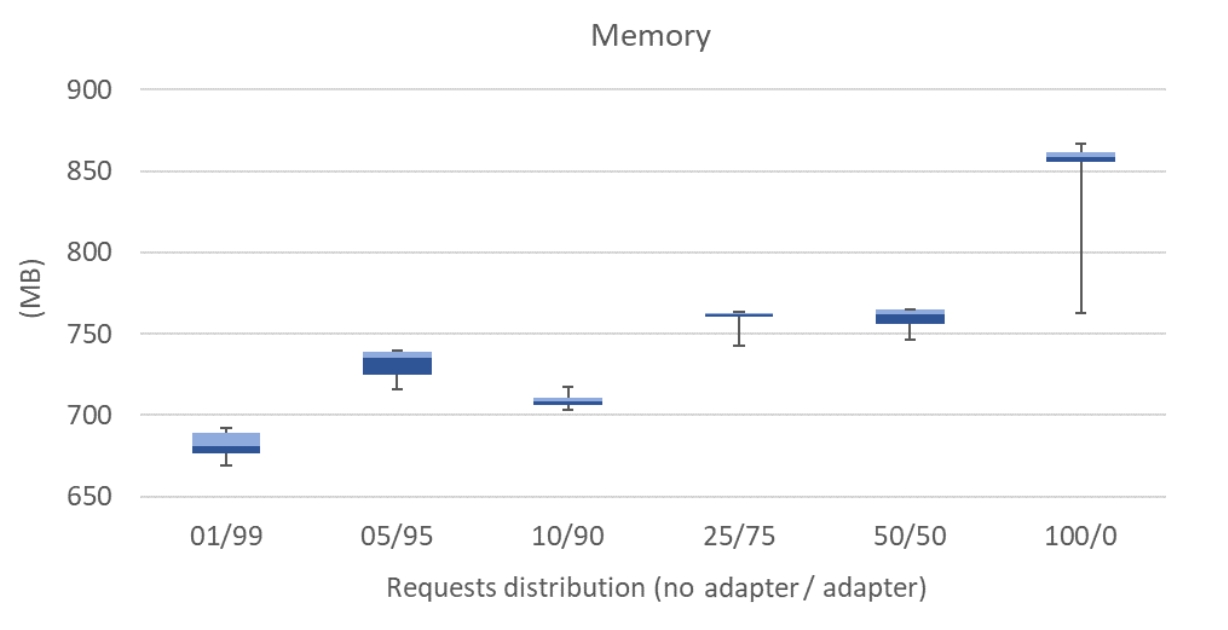
\includegraphics[height=2.9in]{Results/R/Memory-R}}
    \caption{Memory used in the routing experiment - 480 request/s (arrival rate) 100 bytes (payload size)}
    \label{fig:routMem}
\end{figure}

It is expected for the used memory to increase linearly with the fraction of requests routed through the adapter because, as discussed previously,
the adapter implementation spatial complexity is equivalent to double of the demo application implementation spatial complexity.
The results obtained confirm the expectation.

Figure \ref{fig:routLatency} shows the request latency as the proportion of adapted requests increases.
It is expected that the latency will steadily increase, because of the same reasons previously stated.
When comparing the first and last data points, we can see that the latency has doubled as expected.
In the other data points, the latency remains relatively constant, this mainly due to the error introduced by the short test duration.

\begin{figure}[htbp]
    \centering
    \centerline{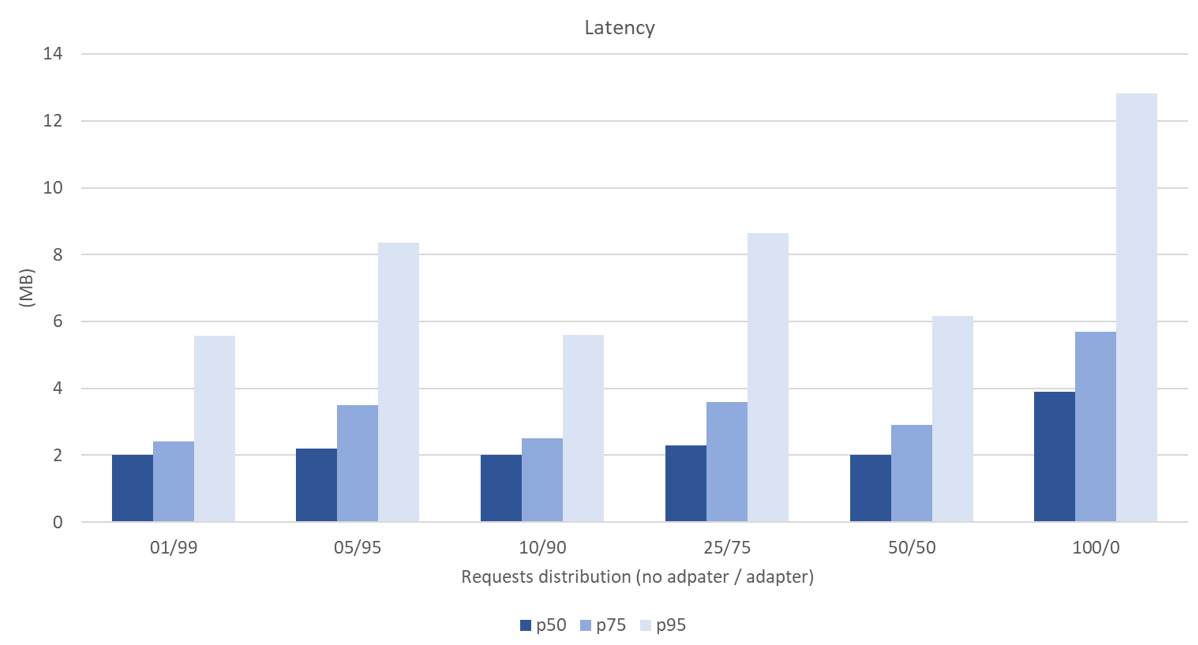
\includegraphics[height=2.9in]{Results/R/Latency-R}}
    \caption{Request latency in the routing experiment - 480 request/s (arrival rate) 100 bytes (payload size)}
    \label{fig:routLatency}
\end{figure}

\subsection{Bi-partition Experiment}

The goal of the experiment was to see if the conclusions obtained from the point-to-point experiment are also applicable in scenarios with multiple microservices.
The experiment is composed by two disjoint sets of microservices, where the first set receives request from the artillery workers and forward the requests to the second of microservices.
The topology is represent in Figure \ref{fig:biPart}.

\begin{figure}[htbp]
    \centering
    \centerline{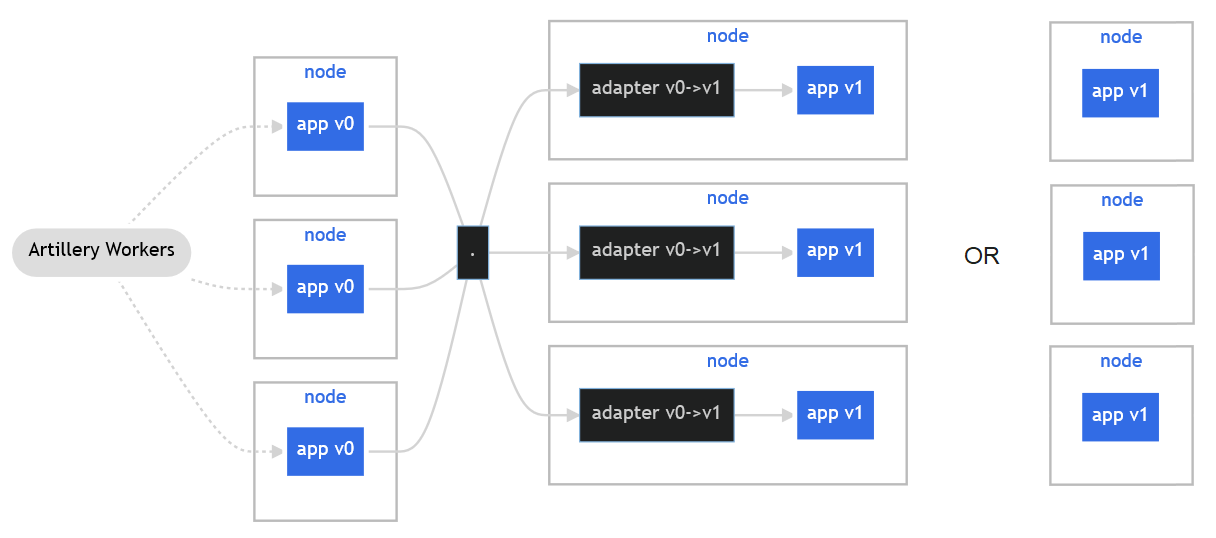
\includegraphics[height=2.6in]{bipartExperiment}}
    \caption{Bi-partition experiment}
    \label{fig:biPart}
\end{figure}

First, it was established a baseline of comparison by doing the tests without the adapter,
then, it was upgraded all the microservices in the second set and added adapters to support communication across the disjoint sets.

The outcomes of the ''point-to-point'' and ''bi-partition'' experiments are equivalent, as seen in the Figures \ref{fig:biPartCPU}, \ref{fig:biPartMem} and \ref{fig:biPartLatency}.

\begin{figure}[htbp]
    \centering
    \centerline{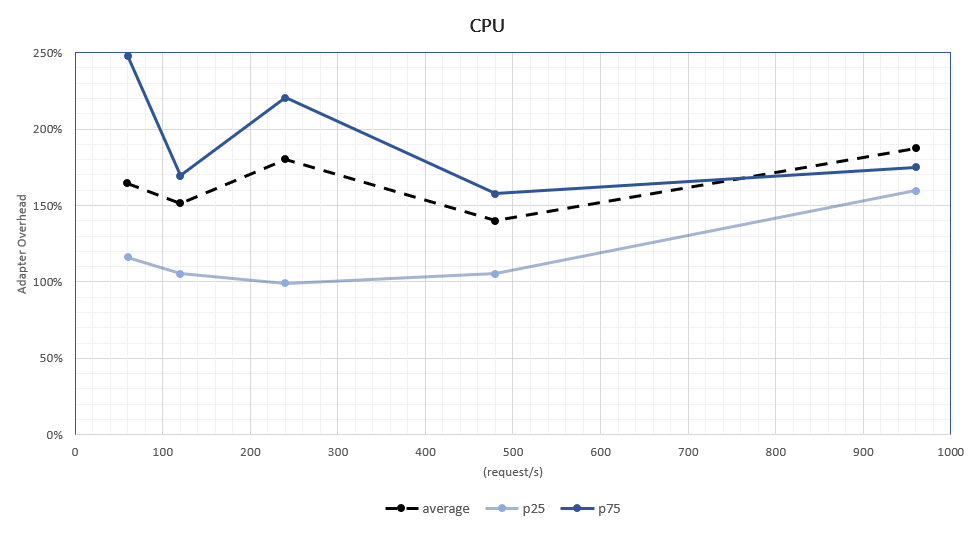
\includegraphics[height=3.2in]{Results/Bp/Cpu-Bp}}
    \caption{Adapter CPU overhead in the bi-partition experiment - 100 bytes (payload size)}
    \label{fig:biPartCPU}
\end{figure}

\begin{figure}[htbp]
    \centering
    \centerline{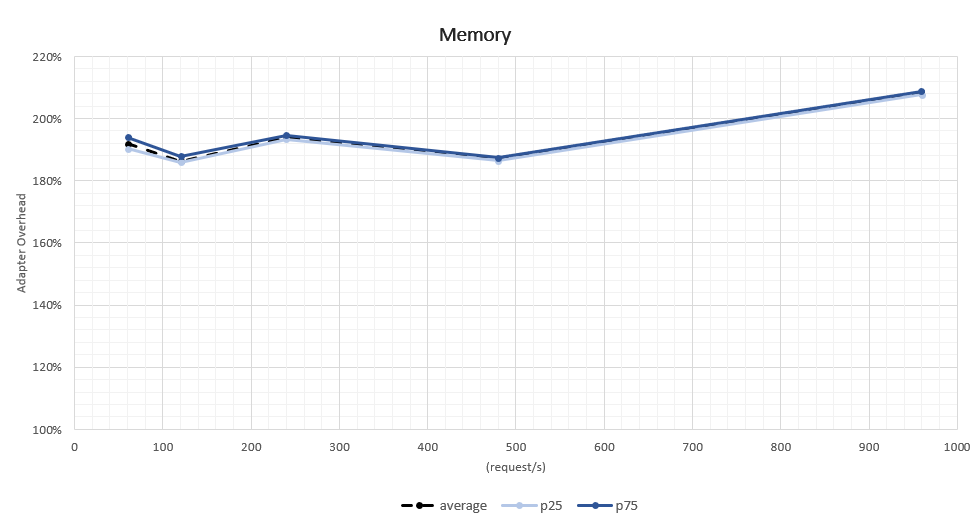
\includegraphics[height=3.3in]{Results/Bp/Memory-Bp}}
    \caption{Adapter memory overhead in the bi-partition experiment - 100 bytes (payload size)}
    \label{fig:biPartMem}
\end{figure}

\begin{figure}[htbp]
    \centering
    \centerline{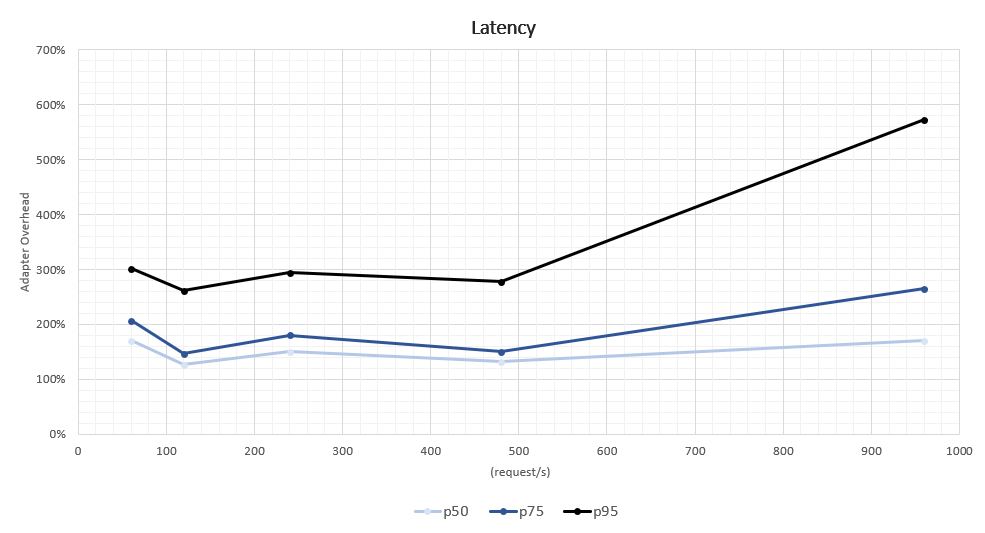
\includegraphics[height=3.2in]{Results/Bp/Latency-Bp}}
    \caption{Adapter latency overhead in the bi-partition experiment - 100 bytes (payload size)}
    \label{fig:biPartLatency}
\end{figure}

\subsection{Live Contract Evolution Experiment}

The experiment's goal was to see if a service's throughput would decrease during a contract upgrade.

The test was performed with the same topology as in the point-to-point experiment.
A deployment operation, was started at minute 2, and finished at minute 3.
In this deployment the proxy adapter was updated, and the contract of one of the services was changed without updating the consumer services.

The deployment was made with a rolling update strategy that incrementally updates pod instances with new ones.
The error rate and timeouts during the experiment were zero.
The experiment was done with an arrival rate of 960 virtual users/second.
Multiple arrival rates were tested, it was selected the highest rate that didn't saturate the application and adapter servers.

The measured results are depicted in Figure \ref{fig:throughputlive}, demonstrating that there is no change in throughput.
There was no change, as expected, because the rolling update strategy deletes previous pods only when new pods are active and reachable.